\documentclass[a4paper,12pt, oneside]{book}

\usepackage{graphicx}
\usepackage{subfigure}
\usepackage{hyperref}
\usepackage[T1]{fontenc}
\usepackage[utf8]{inputenc}
\usepackage{setspace}
\usepackage[paper=a4paper,margin=1in]{geometry}
\usepackage{float}
\usepackage{svg}
\usepackage{amsmath}



% Per Intestazione 
\usepackage{fancyhdr}
\setlength{\headheight}{15pt}
\pagestyle{fancy}
\fancyhead[LO]{\nouppercase{\leftmark}}
\fancyhead[RO]{\nouppercase\rightmark}

\usepackage{minted}
\usemintedstyle{borland}

\usepackage{csquotes}
\usepackage[italian]{babel}

\usepackage[backend=biber, sorting=none]{biblatex}

\usepackage{listings}
\usepackage{pacchetti/protobuf/lang}  % include language definition for protobuf
\usepackage{pacchetti/protobuf/style} % include custom style for proto declarations.

\addbibresource{bibliography.bib}
\addbibresource{web.bib}

\begin{document}


    
    \begin{titlepage}
        
        \noindent
        \begin{minipage}[t]{0.19\textwidth}
            \vspace{-4mm}{
\includegraphics[scale=1.15]{images/logo_unimib.pdf}}
        \end{minipage}
        \begin{minipage}[t]{0.81\textwidth}
        {
                \setstretch{1.42}
                {\textsc{Università degli Studi di Milano - Bicocca}} \\
                \textbf{Scuola di Scienze} \\
                \textbf{Dipartimento di Informatica, Sistemistica e Comunicazione} \\
                \textbf{Corso di laurea in Informatica} \\
                \par
        }
        \end{minipage}
        
	\vspace{40mm}
        
	\begin{center}
            {\LARGE{
                    \setstretch{1.2}
                    \textbf{Sistema di controllo  \\ per base robotica outdoor}
                    \par
            }}
        \end{center}
        
        \vspace{50mm}

        \noindent
        {\large \textbf{Relatore:} Prof. Domenico Giorgio Sorrenti } \\

        \noindent
        {\large \textbf{Correlatore:} Dott. Simone Fontana}
        
        \vspace{15mm}

        \begin{flushright}
            {\large \textbf{Relazione della prova finale di:}} \\
            \large{Federica Di Lauro} \\
            \large{Matricola 829470} 
        \end{flushright}
        
        \vspace{40mm}
        \begin{center}
            {\large{\bf Anno Accademico 2019-2020}}
        \end{center}

        \restoregeometry
        
    \end{titlepage}
    

\begin{titlepage}
\begin{flushright}
	\textit{ma rompi tutto! \\
            hai rotto l'elettricità \\
            ora è un casino}
\end{flushright}

\end{titlepage}
\newpage

\tableofcontents

\newpage

\chapter{Introduzione}

L'obiettivo di questo stage è stato lo sviluppo del sistema di controllo per una base robotica outdoor. Per sistema di controllo intendiamo il software che interagisce con sensori ed attuatori del robot per effettuare il controllo dei motori e ricevere i dati dei sensori ad essi collegati. Oltre al sistema di basso livello è stato inoltre necessario integrare il sistema di controllo sviluppato con il framework ROS (Robot Operating System) per poter scambiare messaggi con un computer, in modo da comunicare ad esso i dati dei sensori e ricevere i comandi per impostare le velocità dei motori.

Il sistema deve rispettare vincoli real-time e garantire stabilità e robustezza del controllo. È inoltre necessario garantire una comunicazione affidabile tra microcontrollore e computer.

Il lavoro è stato articolato nelle seguenti fasi:

\begin{enumerate}
    \item \textbf{Ricerca e installazione dell'hardware}. La base robotica presente in laboratorio IRALab non era completa, in quanto mancavano alcune componenti elettroniche. È stato quindi necessario innanzitutto scegliere e acquistare il nuovo hardware, e procedere con l'installazione a bordo del robot.
    \item \textbf{Analisi dei requisiti e progettazione}. È stata fatta un'analisi dei requisiti per garantire i vincoli sopraelencati ed è stata effettuata un'adeguata progettazione del software, sia per quanto riguarda il microcontrollore che per il nodo ROS.
    \item \textbf{Sviluppo software microcontrollore}. È stato sviluppato il software per poter leggere i sensori, controllare i motori ed effettuare la comunicazione con il computer.
    \item \textbf{Sviluppo nodo ROS}. È stato sviluppato un nodo ROS per poter fare da ponte tra il microcontrollore e il framework ROS
    \item \textbf{Testing}. Il sistema di controllo è stato testato dal vivo, comandando il robot con un joypad.
\end{enumerate}

\chapter{Strumenti}

\section{ROS}

ROS (Robot Operating System) è un framework flessibile usato per scrivere software per robot.
È una collezione di strumenti, librerie e convenzioni che ha lo scopo di semplificare la creazione di sistemi robot complessi e robusti in modo indipendente dalla piattaforma robotica.

ROS è costituito da una rete di processi che vengono eseguiti in parallelo e comunicano tra di loro in modo Peer-to-Peer.
Gli elementi principali che costituiscono il sistema sono:
\begin{itemize}
  \item \textbf{Nodi}: sono i processi che vengono eseguiti in parallelo.
  \item \textbf{Master}: è il server principale che si occupa di effettuare le operazioni di routing per permettere la comunicazione tra i diversi nodi.
  \item \textbf{Messaggi}: il contenuto che si scambiano i nodi. I messaggi possono essere sia di tipo standard sia definiti in modo custom.
  \item \textbf{Topic}: sono il canale di comunicazione usato dai nodi per permettere lo scambio di messaggi.
\end{itemize}
Il sistema di scambio dei messaggi si basa sull'architettura publisher/subscriber: ogni nodo può essere \textit{talker} (Publisher) o \textit{listener}  (Subscriber).
Un nodo talker può creare topic e pubblicare i messaggi su questi canali (sia su topic creati dal nodo steso, sia su topic già esistenti), mentre un nodo listener si sottoscrive ai topic ed esegue una callback ogni volta che viene ricevuto un messaggio. Più nodi listener si possono sottoscrivere allo stesso topic e più nodi talker possono pubblicare sullo stesso topic.

Il software è open source ed è disponibile sul sito ufficiale \cite{ROS}, la versione usata per questo progetto è la Melodic.

\begin{figure}[H]
\centering
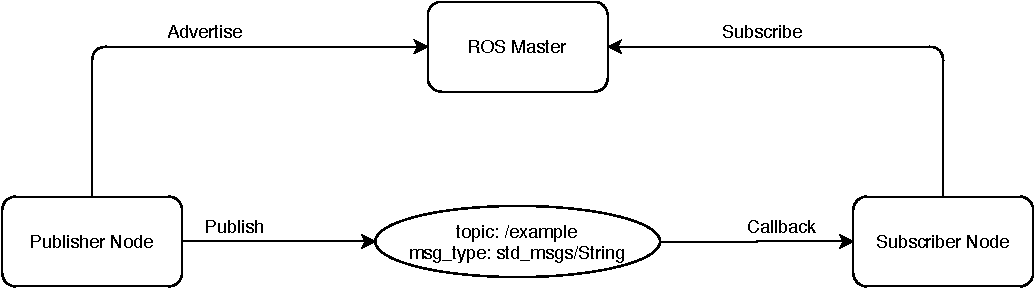
\includegraphics[width=\textwidth]{images/ros_system.pdf}
\caption{Schema generale del sistema di comunicazione}
\end{figure}

\section{RVIZ}
RVIZ è un tool che permette la visualizzazione 3D dei messaggi scambiati da ROS. Usando questo strumento si può visualizzare in real-time la posizione del robot attraverso i dati dei sensori che vengono pubblicati.

\begin{figure}[H]
\centering
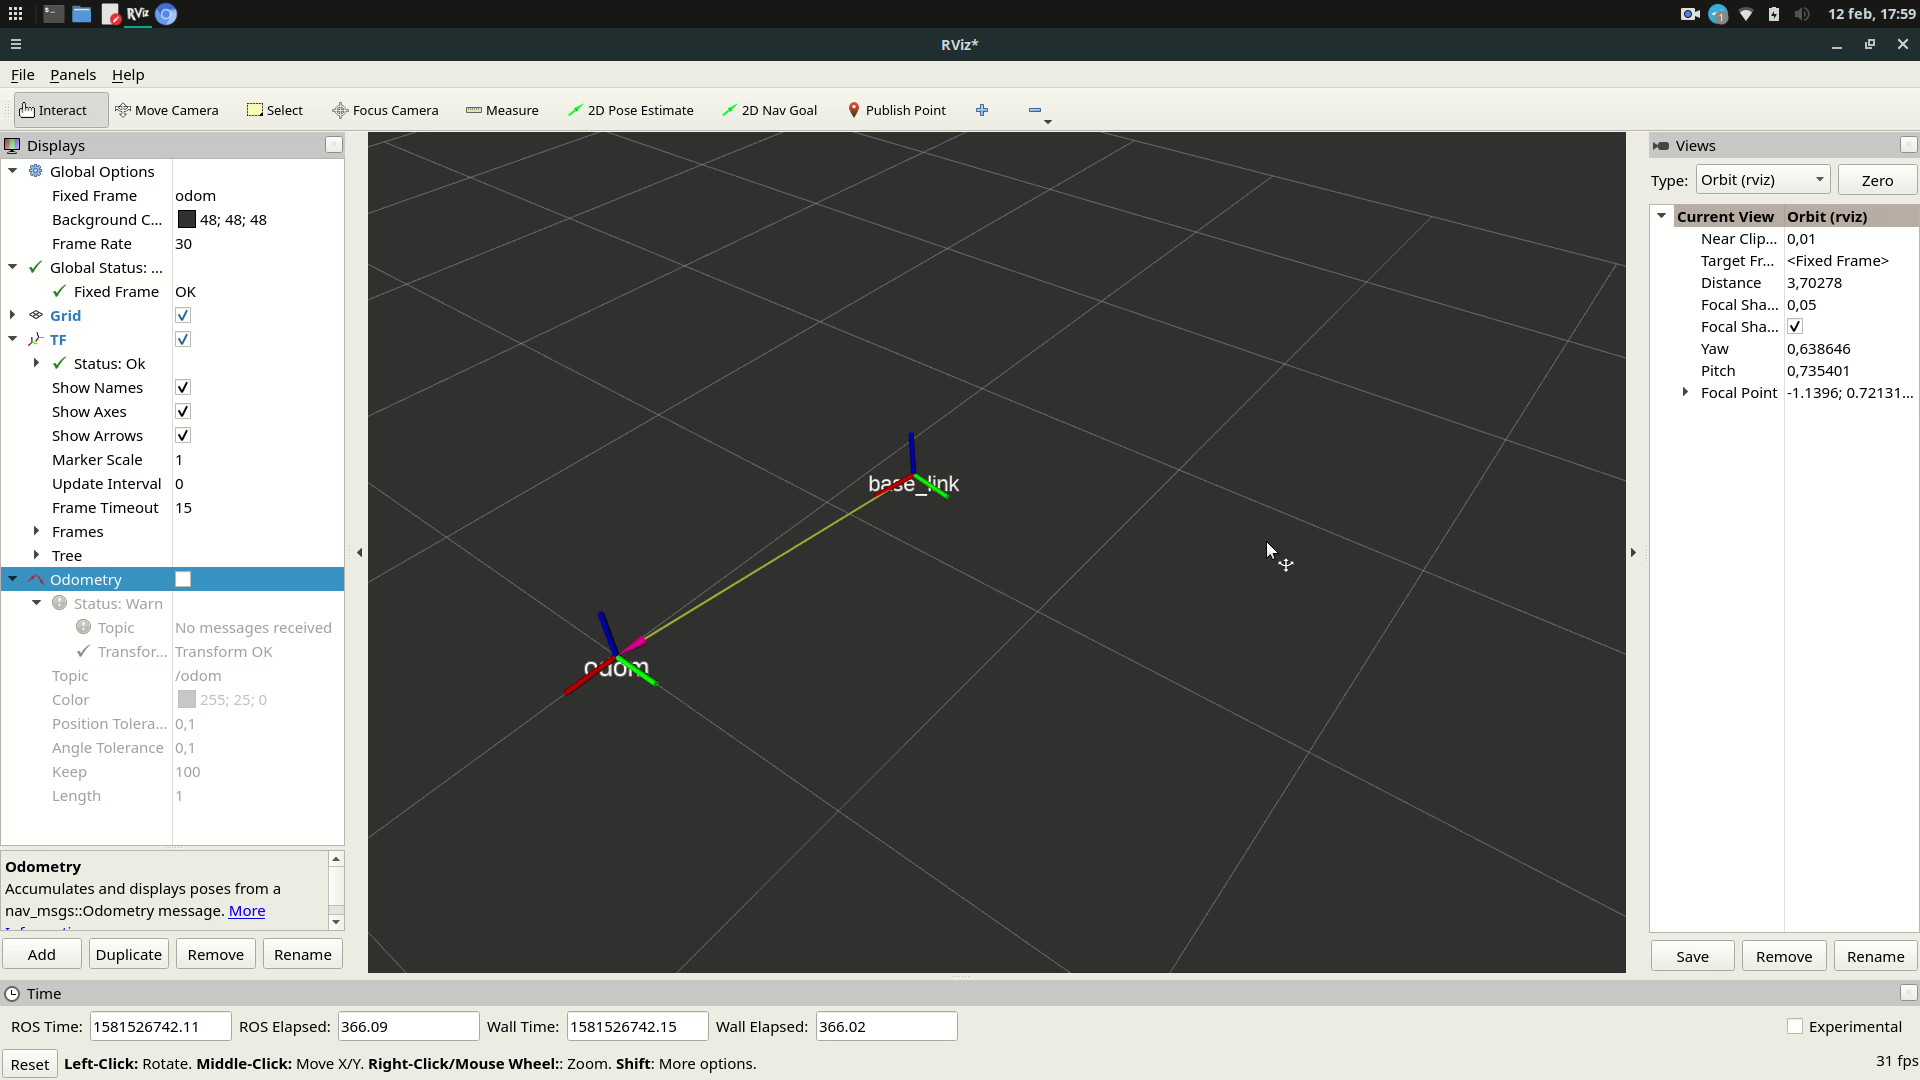
\includegraphics[width=\textwidth]{images/rviz.png}
\caption{Visualizzazione di un robot nello spazio con RVIZ}
\end{figure}

\section{STM32CubeIDE}
STM32CubeIDE è un ambiente di sviluppo della ST Microelectronics per la programmazione e il debugging delle schede STM32. Il software è scaricabile gratuitamente dal sito ufficiale \cite{STM32CubeIDE}. \\
Le sue principali caratteristiche sono:
\begin{itemize}
    \item Toolchain GNU C/C++ per Arm e GDB debugger.
    \item Integrazione del tool STM32CubeMX per la generazione del codice di configurazione del sistema e delle periferiche del microcontrollore.
    \item Debugging avanzato che comprende feature come:
    \begin{itemize}
        \item Visualizzazione di CPU core, registri delle periferiche e memoria
        \item Visione delle variabili live 
        \item Analisi del sistema e tracing in tempo reale
        \item Tool di analisi dei CPU fault
    \end{itemize}
\end{itemize}

\begin{figure}[H]
\centering
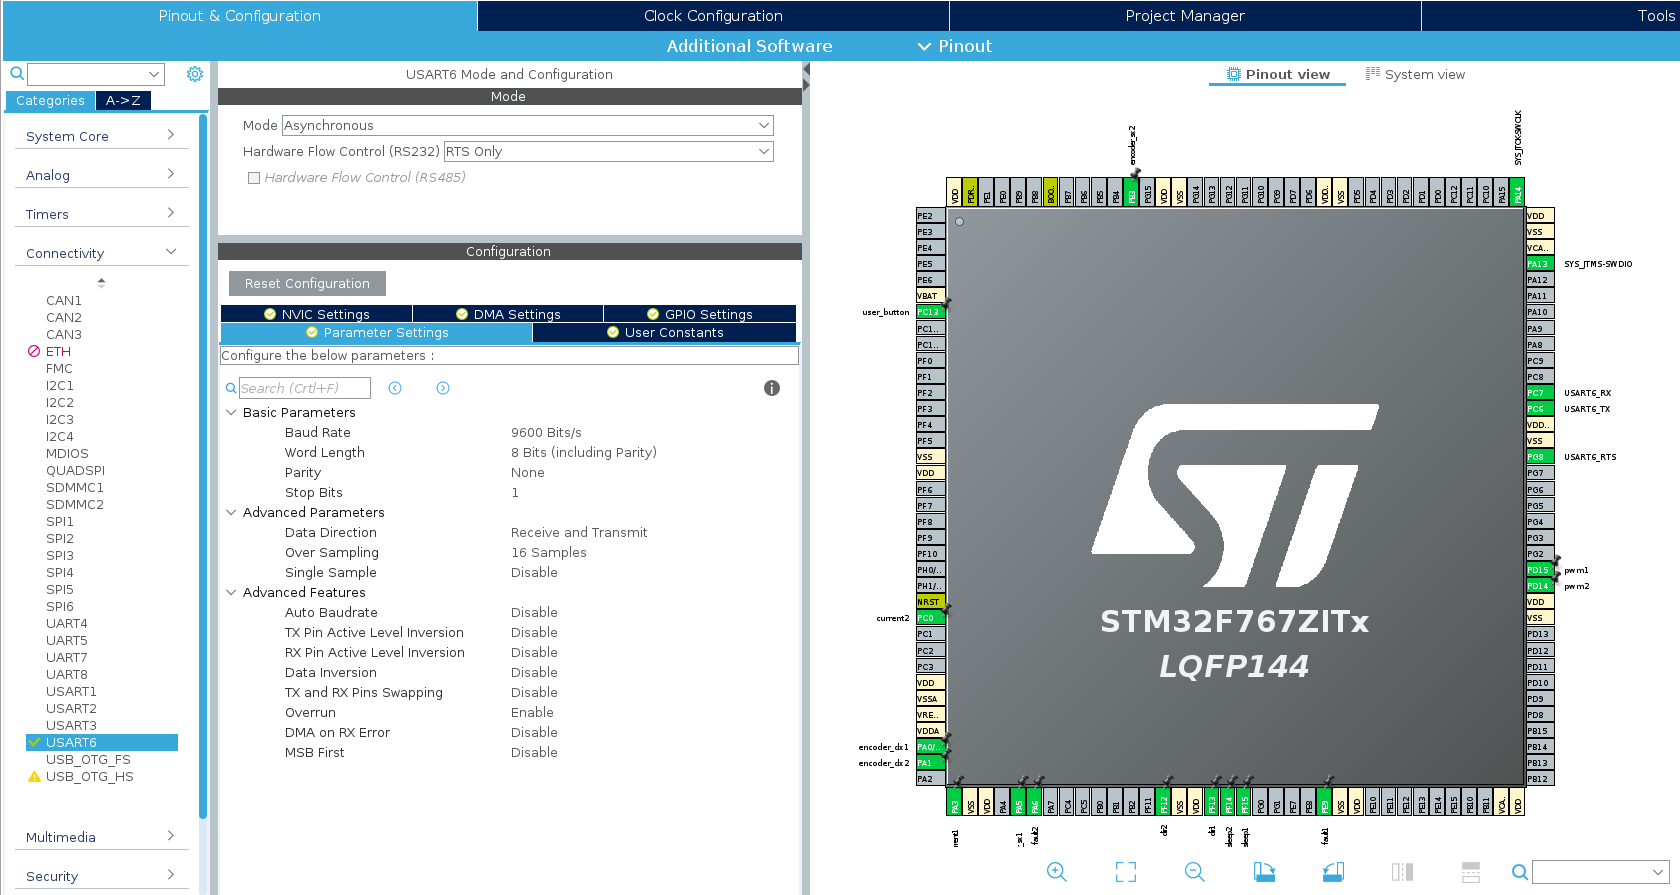
\includegraphics[width=\textwidth]{images/stm32cubemx.png}
\caption{Configurazione di pinout e periferiche tramite lo strumento STM32CubeMX}
\end{figure}

\section{Protocol Buffers}
Protocol Buffers è una libreria per la serializzazione dei dati strutturati, utile per lo sviluppo di software che necessita uno scambio di informazioni tra sistemi indipendenti.
La struttura dei dati viene descritta in un file di tipo \textit{.proto}, dopo di che, attraverso la compilazione con il comando \textit{protoc} e specificando il linguaggio di programmazione desiderato, vengono generate le classi per accedere ai dati. 
                
Protocol Buffers è sviluppato da Google e rilasciato con licenza open source \cite{ProtocolBuffers}. \\
Per questo progetto è stata utilizzata anche un'implementazione in C pensata per i microcontrollori, \textit{nanopb} \cite{nanopb}.

\newpage

\lstinputlisting[language=protobuf2, 
                style=protobuf,
                caption={Esempio di definizione di un messaggio con Protocol Buffers},
                captionpos=b]{codice/esempio.proto}


\section{sigrok Pulseview}
sigrok è una suite di software per l'analisi dei segnali, sfruttando dispositivi come oscilloscopi e analizzatori logici. 

Pulseview è l'interfaccia grafica usata per sfruttare questi tool e permette di interfacciarsi con i dispositivi sopracitati visualizzando il segnale in tempo reale, analizzandone i tempi e consente inoltre la decodifica di segnali digitali. 

In particolare per questo progetto è stato usato Pulseview con un analizzatore logico per facilitare il debugging nella trasmissione dei segnali, ad esempio la trasmissione seriale di messaggi.

\begin{figure}[H]
\centering
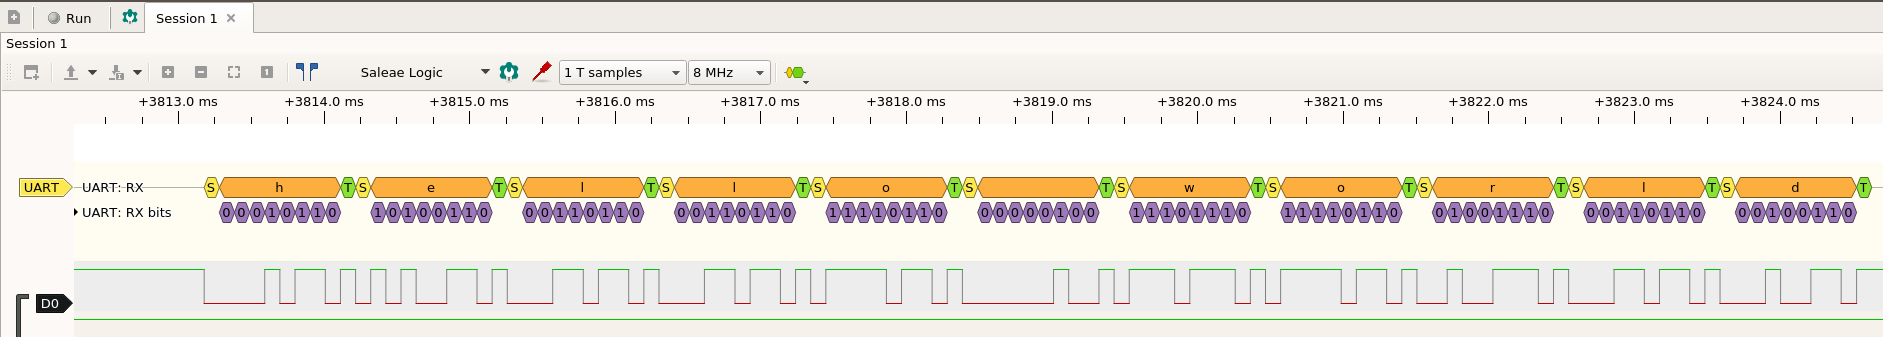
\includegraphics[width=\textwidth]{images/pulseview.png}
\caption{Acquisizione e decodifica di un segnale UART}
\end{figure}

Pulseview è un progetto open source e liberamente scaricabile dal sito ufficiale\cite{Pulseview}.
\chapter{Base robotica Otto}

Otto è un robot a guida differenziale, progetto di ricerca del laboratorio di robotica IRALab, dell’Università degli Studi di Milano-Bicocca.

\section{Base robotica VolksBot RT 3}
VolksBot è un kit modulare per la costruzione di robot, progettato per il campo della ricerca e della  prototipazione rapida.
La base robotica è pensata per essere facilmente modificata ed adattata alle proprie esigenze in quanto composta da barre in alluminio combinabili fra di loro.

Nello specifico la base robotica utilizzata è composta da due ruote motrici frontali e una ruota basculante di supporto posteriore.
Ciascuna ruota motrice è collegata ad un motore a corrente continua combinato con una riduzione con un rapporto di trasmissione 1:74.
L'intero sistema robotico è alimentato tramite batterie a bordo del veicolo.
\begin{figure}[H]
\centering
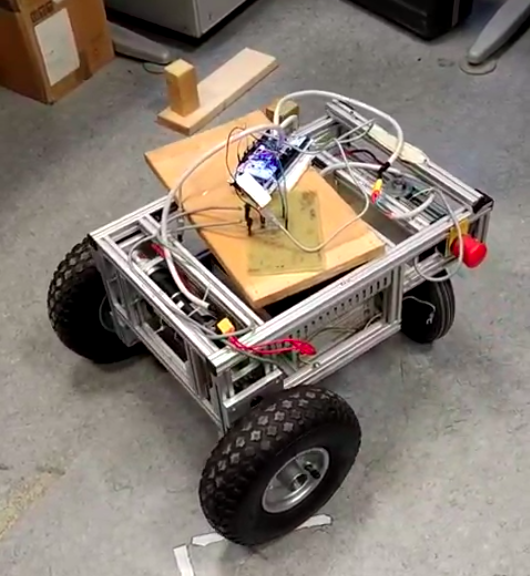
\includegraphics[scale=0.45]{images/otto1.png}
\caption{Base robotica Otto}
\end{figure}

\section{Encoder}
Un encoder è dispositivo elettromeccanico in grado di convertire la posizione o il moto angolare in un codice digitale.

Nel nostro caso è stato montato un encoder in quadratura sull'asse del motore di ciascuna ruota motrice.
Questo tipo di sensore è formato da un LED, da una corona circolare con un pattern fisso che si ripete e da dei fotodiodi. 

\begin{figure}[H]
\centering
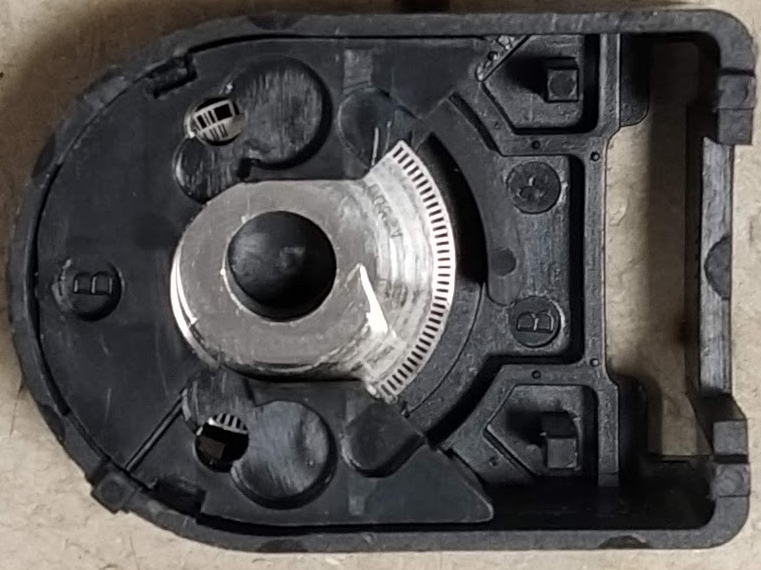
\includegraphics[scale=0.30]{images/corona.png}
\caption{Corona circolare dell'encoder}
\end{figure}

Il funzionamento si basa sulla capacità dei fotodiodi di percepire i cambiamenti di luce: il LED viene sempre alimentato ed emette quindi una luce costante, la corona dell'encoder gira insieme all'albero del motore e i fotodiodi rilevano i cambiamenti di luce dovuti al pattern sulla corona e tramite dei comparatori generano delle onde quadre.
Elaborando questi segnali è possibile misurare sia la distanza percorsa dalle ruote che la direzione del movimento.

\begin{figure}[H]
\hfill
\subfigure[Schema dell'encoder]{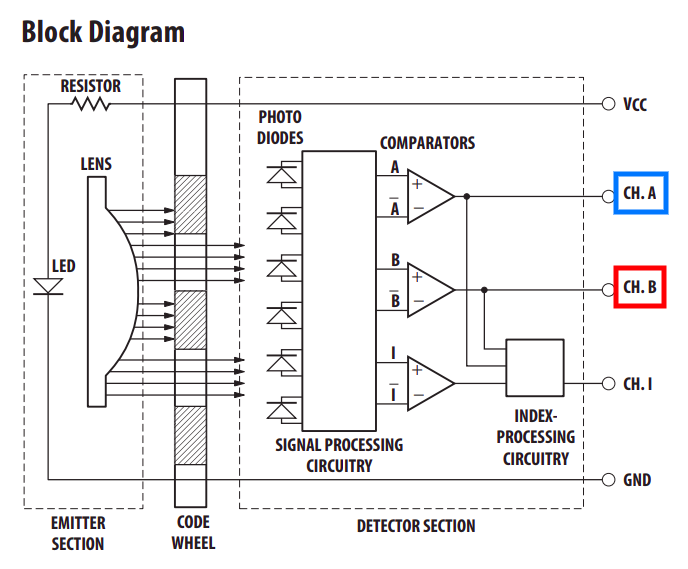
\includegraphics[scale=0.32]{images/encoder-1.png}}
\hfill
\subfigure[Segnale generato]{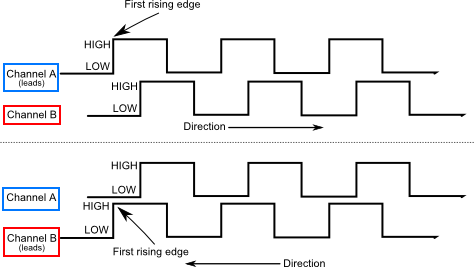
\includegraphics[scale=0.47]{images/quad-encoding-waveform-1.png}}
\hfill
\caption{Encoder in quadratura}
\end{figure}

\section{Motor driver}
Un motor driver è un dispositivo elettronico necessario per poter controllare i motori DC usando i segnali digitali generati da un microcontrollore.
Il circuito elettronico principale è chiamato ponte H e permette di controllare la polarità della tensione applicata a un carico. Tramite questo meccanismo siamo in grado sia di controllare la direzione del moto di un motore a corrente continua, stabilendo il verso nel quale fluisce la corrente, sia di regolare la velocità del motore modulando la tensione.

La modulazione della tensione avviene tramite un segnale PWM (pulse-width modulation). Questo segnale periodico ha due fasi: una in cui la tensione è alta (3.3V) e una fase in cui la tensione è bassa (0V). Il rapporto tra queste due fasi è detto duty-cycle e determina la tensione media in uscita.

\begin{figure}[H]
\centering
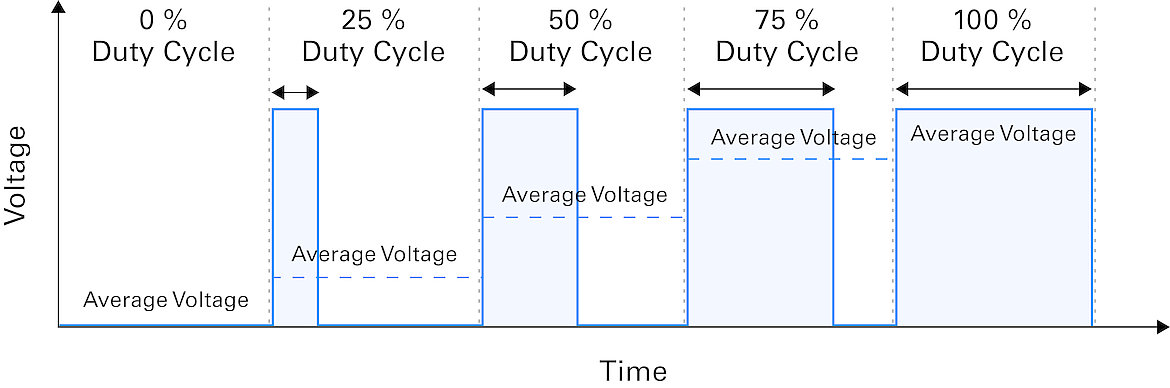
\includegraphics[width=\textwidth]{images/pwm.jpg}
\caption{Modulazione della tensione con segnale PWM.}
\end{figure}


Il motor driver scelto è Pololu Dual G2: questo dispositivo ha due circuiti H-bridge, così da poter controllare entrambi i motori in modo indipendente.
Per controllare ciascun motore sono presenti 3 segnali di input:
\begin{itemize}
    \item SLP: disabilita l'output se è uguale a 0
    \item PWM: input particolare rappresentabile come percentuale, modula la velocità
    \item DIR: imposta la direzione di azione del motore
\end{itemize}

Si hanno quindi le seguenti modalità di funzionamento:
\begin{table}[H]
    \centering
    \begin{tabular}{|l|l|l|l|}
    \hline
    SLP & DIR & PWM & Operazione                            \\ \hline
    1   & 0   & \%pwm & motore azionato in senso orario a velocità pwm \\
    1   & 1   & \%pwm & motore azionato in senso antiorario a velocità pwm         \\
    1   & x   & 0   & motore frenato                        \\
    0   & x   & x   & motore libero                     \\ \hline
    \end{tabular}
\end{table}

Sono inoltre presenti due segnali analogici di output per controllare il consumo dei motori (CS) e due segnali di output per monitorare lo stato di eventuali guasti (FLT).

\begin{figure}[H]
\centering
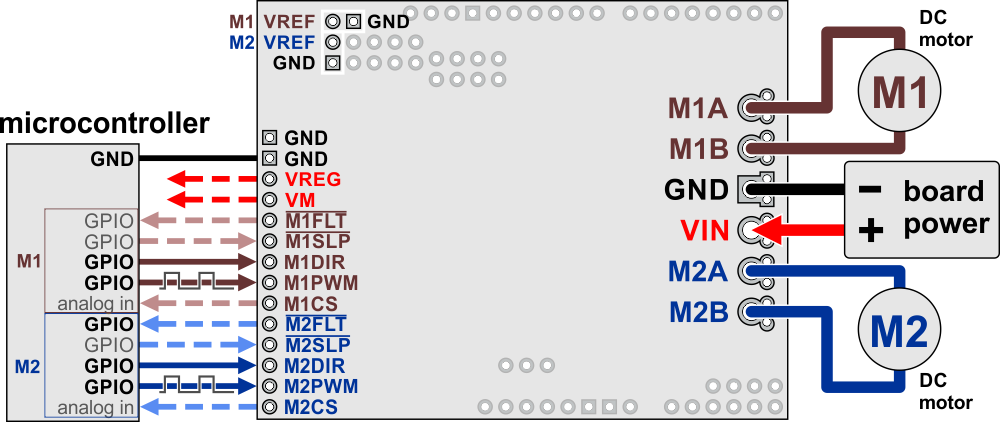
\includegraphics[scale=1.4]{images/pololu.png}
\caption{Schema delle connessioni del Pololu Dual G2.}
\end{figure}


\section{Microcontrollore}
La scheda di sviluppo scelta è una Nucleo STM32F767ZI.
Il processore è un Core Arm 32-bit Cortex-M7, ed è presente una Floating Point Unit per velocizzare le operazioni in virgola mobile.
La scheda ha 512kB di memoria RAM e 2MB di memoria FLASH.
È stata scelta per la grande disponibilità di periferiche integrate, in particolare per la realizzazione del sistema di controllo sono stati necessari: 
\begin{itemize}
    \item 2 timer a 32 bit per la gestione degli encoder.
    \item 1 timer a 16 bit per la generazione del segnale PWM.
    \item 1 periferica UART per la comunicazione con il computer.
\end{itemize}
Inoltre è presente un debugger integrato ST-LINK V2.1.

\begin{figure}[H]
\centering
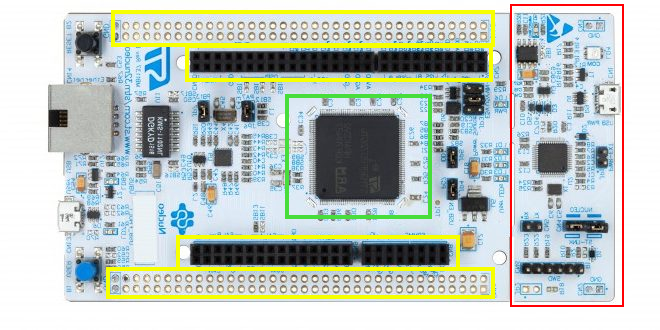
\includegraphics[scale=0.65]{images/nucleo.png}
\caption{La scheda Nucleo. Evidenziato in rosso il debugger, in verde il processore ed in giallo i GPIO per interfacciarsi con le varie periferiche.}
\end{figure}

\section{Modulo FTDI}
Per quanto riguarda la comunicazione tra microcontrollore e computer si è scelto il protocollo UART. 
Per rendere il sistema utilizzabile collegando un qualsiasi computer è stato necessario un modulo apposito che convertisse il segnale UART in un segnale USB, così da non dover utilizzare una piattaforma apposita dotata di GPIO.

È stato utilizzato un modulo FTDI FT232RL in quanto ampiamente supportato a livello di driver Linux e perché, oltre alle linee di trasmissione e ricezione, presenta alcuni meccanismi di controllo del flusso hardware tramite appositi pin (CTS e RTS) e un pin per poter effettuare il reset del microcontrollore direttamente dal PC.


\begin{figure}[H]
\centering
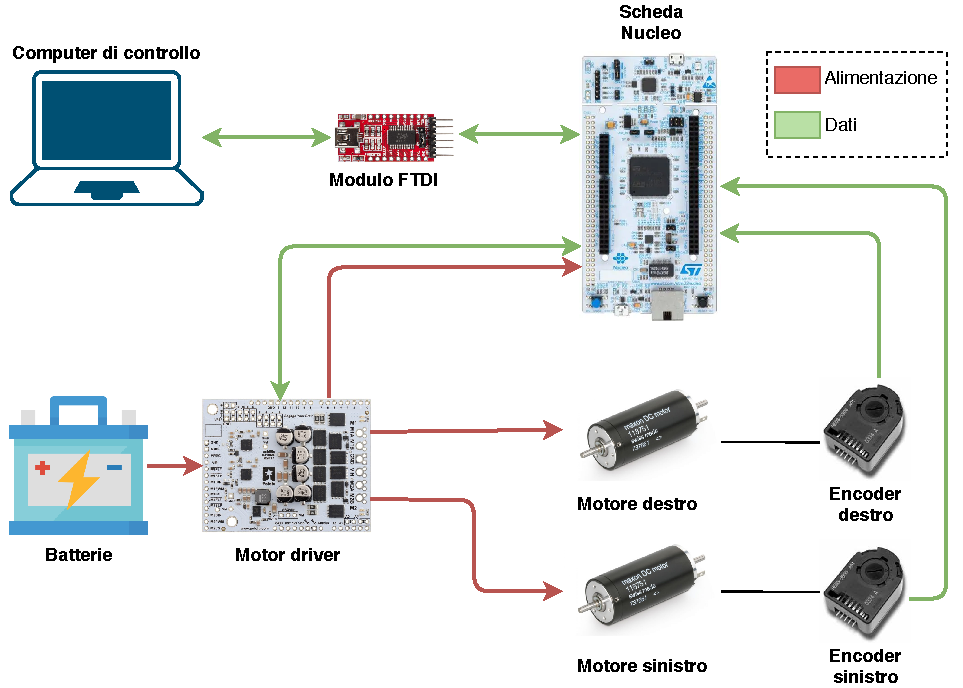
\includegraphics[width=\textwidth]{images/infrastruttura.pdf}
\caption{Riepilogo generale dei componenti e delle loro connessioni.}
\end{figure}

\chapter{Sviluppo}

\section{Progettazione del sistema}
L'obiettivo di questo stage è stato la creazione del sistema di controllo di un robot a guida differenziale che si integrasse con il framework ROS.
Innanzitutto è stata necessaria un'analisi dei requisiti, nella quale sono stati individuati i seguenti punti: 
\begin{itemize}
    \item Elaborazione dei dati degli encoder per ricavare l'odometria del robot.
    \item Controllo dei motori tramite un sistema in retroazione.
    \item Comunicazione bidirezionale con un computer di controllo.
\end{itemize}

Per l'ultimo punto è stato necessario studiare un sistema per poter integrare la comunicazione con il framework ROS, in particolare per poter utilizzare il Navigation Stack.
Lo stack di navigazione è molto semplice a livello concettuale. Esso riceve le informazioni riguardanti l'odometria e i dati dei sensori, e restituisce in output i comandi che il robot deve eseguire.

\begin{figure}[h]
    \centering
    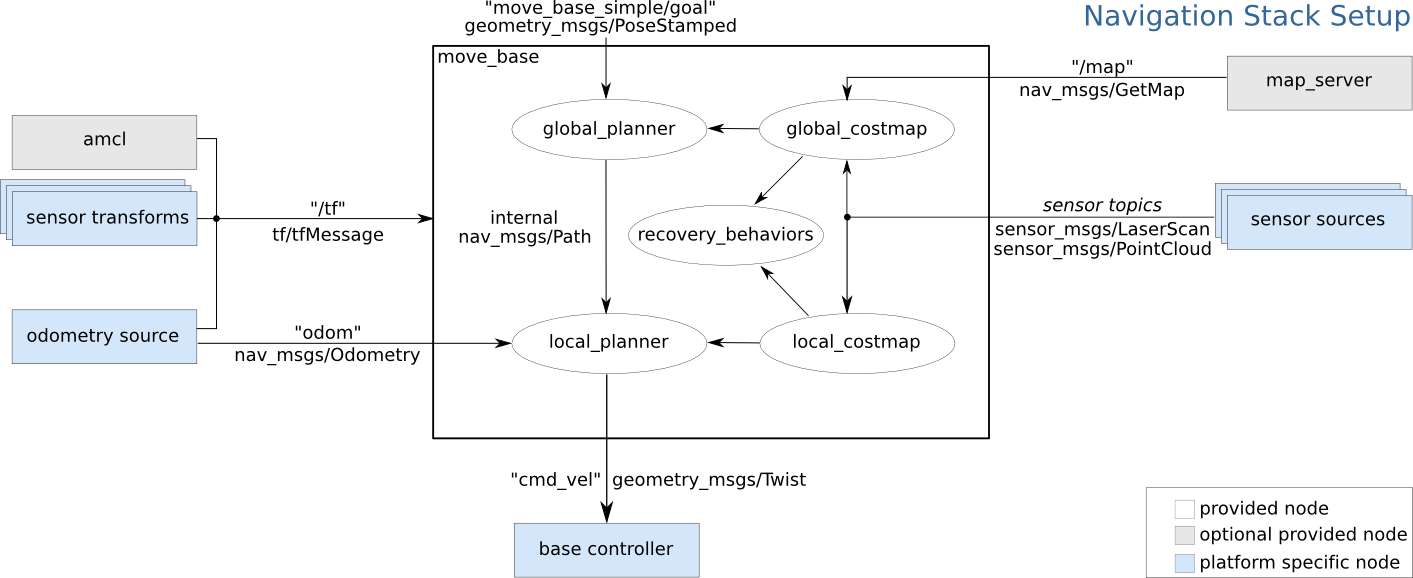
\includegraphics[width=\textwidth]{images/navigation_stack.png}
    \caption{Lo schema dello stack di navigazione. Come mostrato nella legenda, i nodi in
bianco sono quelli già forniti, quelli in grigio sono opzionali e quelli in blu sono specifici per il singolo robot che devono essere implementati.}
  \label{fig:navigation_stack}
\end{figure}

\newpage
Come illustrato nella figura \ref{fig:navigation_stack} i messaggi da pubblicare, per quanto riguarda il sistema di controllo, sono messaggi di tipo \textit{nav\_msgs/Odometry} sul topic \textit{/odom} e messaggi di tipo \textit{tf/Message} sul topic \textit{/tf}; bisogna sottoscriversi ai messaggi di tipo \textit{geometry\_msgs/Twist} sul topic \textit{/cmd\_vel}. \\
Il messaggio \textit{Odometry} contiene le informazioni riguardanti la pose del robot nello spazio, prendendo come sistema di riferimento la prima pose del robot, ed è composto da:
\begin{itemize}
    \item Posizione espressa come \textit{x, y, z}
    \item Orientamento espresso come \textit{quaternion}
    \item Velocità lineare e velocità angolare attuali
\end{itemize}

Il messaggio \textit{tf} contiene le informazioni riguardanti la pose del robot ed è necessario in quanto ci permette di rappresentare l'albero delle trasformazioni delle varie parti del robot, ovvero le posizioni relative delle varie parti come laser e altri sensori rispetto alla base mobile, chiamata \textit{base\_link}.

Il messaggio \textit{geometry\_msgs/Twist} contiene le informazioni per far muovere il robot, nel caso di un robot a guida differenziale queste informazioni sono la velocità lineare sull'asse delle x, e la velocità angolare rispetto all'asse delle z.

Si è scelto di far gestire la parte relativa allo scambio dei messaggi ROS al computer principale, che comunica con la scheda di controllo tramite il modulo usb-seriale. 
È stato creato un nodo ROS, che si sottoscrive al topic \textit{/cmd\_vel} e trasmette i comandi alla scheda, e che riceve le informazioni relative alla velocità del robot, le elabora e pubblica i messaggi su \textit{/odom} e \textit{/tf}.

Il microcontrollore deve svolgere tre compiti: 
\begin{itemize}
    \item Inviare i dati di odometria.
    \item Gestire i loop di controllo PID per la gestione dei motori.
    \item Ricevere i comandi, ricavare i valori delle velocità dei motori e impostare quindi i setpoint dei controlli PID.
\end{itemize}

La trasmissione dei dati di odometria avviene periodicamente leggendo i dati degli encoder, mentre l'aggiornamento dei comandi da far eseguire ai motori avviene in modo asincrono ogni volta che un messaggio di comando viene ricevuto.


\begin{figure}[H]
    \centering
    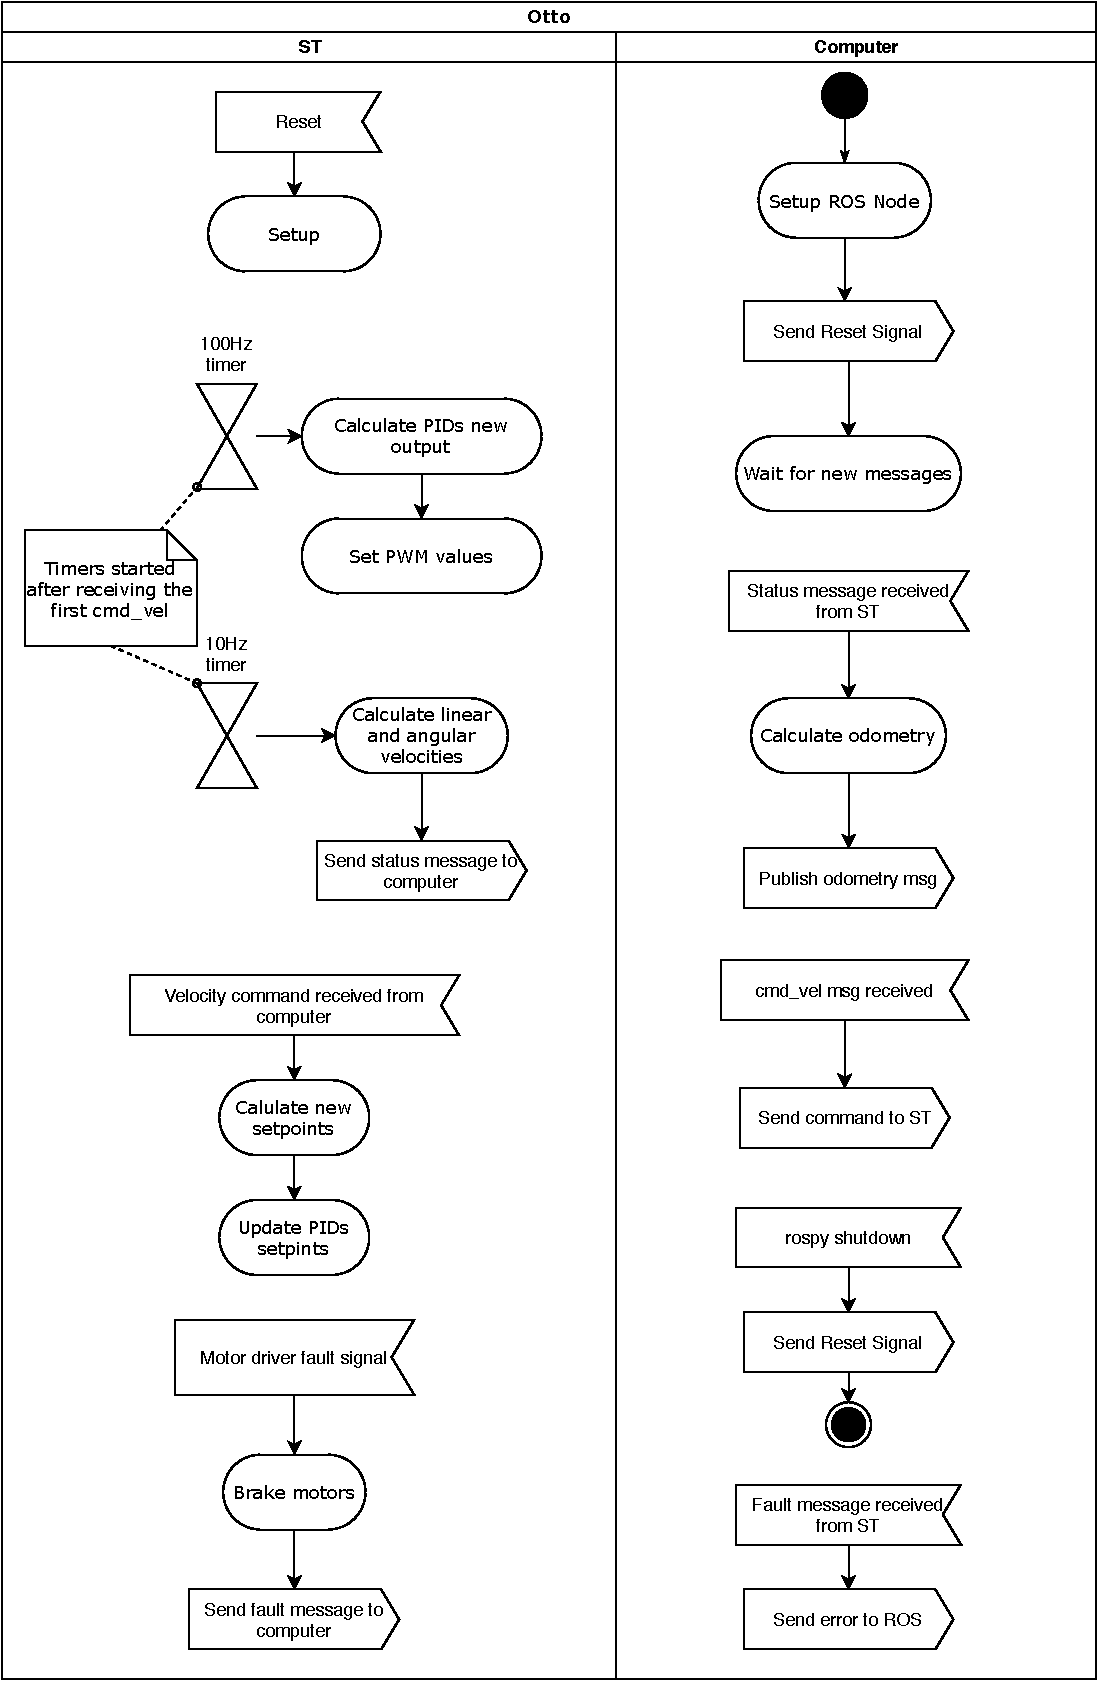
\includegraphics[scale=0.84]{images/uml_activities.pdf}
    \caption{Diagramma delle attività}
\end{figure}
\newpage

\section{Implementazione microcontrollore}
\subsection{Struttura del codice}
Lo scheletro del codice e l'inizializzazione delle periferiche sono stati generati tramite lo strumento STM32CubeMX. 
Il software è stato scritto in C++, piuttosto che in C, per permettere un miglior riutilizzo del codice attraverso l'utilizzo delle classi. In particolare sono state create 4 classi: una per la gestione degli encoder, una per la gestione del ponte H, una per l'odometria e una per il controllo PID.

Il sistema di controllo è basato sugli interrupt: per la gestione dei task periodici, ovvero l'invio dei dati di odometria e il controllo PID dei motori, sono stati usati due timer che generano un interrupt a frequenza fissa (rispettivamente 10Hz per l'invio dell'odometria e 100Hz per il controllo PID), mentre per la ricezione dei comandi dal computer è usato un approccio asincrono: alla ricezione di ogni comando viene lanciato un interrupt. Vengono inoltre utilizzati degli interrupt per la gestione dei guasti dei motori.

Un interrupt è un particolare tipo di eccezione, che viene generata dalle periferiche o dal software in modo asincrono rispetto all'esecuzione del codice.
Un'eccezione può trovarsi in 4 stati:
\begin{itemize}
    \item Inattiva: eccezione non attiva e non in sospeso.
    \item In sospeso (\textit{pending}): eccezione in attesa di essere servita dal processore. Una interrupt request da una periferica può far passare la sua corrispondente eccezione in questo stato. 
    \item Attiva: eccezione che è attualmente servita dal processore ma non è completa.
    \item Attiva e in sospeso: l'eccezione è attualmente servita dal processore, ed è stata generata un'altra eccezione dalla stessa fonte. 
\end{itemize}
Il processore gestisce gli interrupt attraverso Interrupt Service Routines (ISRs): gli indirizzi in memoria di queste ISR sono contenuti nella \textit{vector table}. Nelle librerie di Hardware Abstraction Layer utilizzate all'interno di ogni ISR viene chiamata una funzione di callback, il cui codice è definibile dal programmatore.
Ad ogni eccezione è associato un livello di priorità: il livello 0 è il livello con priorità massima. Il livello di priorità di ogni eccezione è configurabile, tranne per le eccezioni di sistema la cui priorità è fissata a 0.
Se due eccezioni sono in stato pending, verrà servita prima quella con priorità più alta.
Se durante la ISR di un'eccezione viene rilevata un'eccezione con priorità più alta, la ISR dell'eccezione attualmente gestita viene messa in attesa (pre-empted) e viene gestita l'eccezione con priorità più alta.

In particolare la configurazione degli interrupt è effettuata da una particolare periferica, il Nested Vectored Interrupt Controller (NVIC). Attraverso il NVIC è possibile configurare la priorità degli interrupt con un meccanismo aggiuntivo, ovvero dividendo il livello di priorità in \textit{group priority} e in \textit{subpriority}. 
La \textit{group priority} determina il livello di priorità degli interrupt, permettendo di applicare il meccanismo \textit{pre-emptive} illustrato sopra. Se durante la gestione di un interrupt viene rilevato un interrupt con la stessa group priority non viene applicata la pre-emption.
Se più interrupt in sospeso hanno la stessa group priority, la subpriority determina l'ordine nel quale verranno processati.

Sono stati impostati i livelli di group priority e subpriority per garantire il corretto funzionamento del sistema. In particolare il rilevamento di malfunzionamenti dei motori ha priorità massima, segue l'interrupt associato alla ricezione dei messaggi e infine TIM3 e TIM6 hanno la stessa priorità in quanto utilizzano risorse condivise, avendo la stessa priorità non c'è pre-emption e quindi non ci sono criticità legate alla sincronizzazione dei task. I task a priorità diverse non accedono alle stesse risorse, quindi non ci sono problemi legati alla preemption tra task con livelli di priorità diverse.

\begin{table}[H]
\centering
\begin{tabular}{lll}
\hline
\textbf{Interrupt} & \textbf{Group priority} & \textbf{Subpriority} \\ \hline
EXTI[9:5]          & 0                       & 0                    \\ \hline
USART6             & 1                       & 0                    \\ \hline
TIM3               & 2                       & 1                    \\ \hline
TIM6               & 2                       & 2                    \\ \hline
\end{tabular}
\end{table}

Per utilizzare un timer per la generazione periodica di interrupt lo si imposta come \textit{time base generator}. Ogni timer è collegato tramite un bus ad un clock, la frequenza di questo clock può poi essere divisa da un prescaler, il cui valore è specificato nel registro TIMx\_PSC. Il timer in questa modalità incrementa di 1 il suo registro TIMx\_CNT ad ogni pulsazione del clock diviso dal prescaler; quando il valore nel registro TIMx\_CNT è uguale al valore registro TIMx\_ARR il valore di TIMx\_CNT viene azzerato e viene generato un interrupt \cite{STM32_timer_cookbook}.
Si può calcolare la frequenza alla quale viene generato l'interrupt con la seguente formula:
\begin{displaymath}
Interrupt frequency = \frac{TIMx\_CLOCK}{(TIMx\_PSC + 1)*(TIMx\_ARR + 1)}
\end{displaymath}
In particolare, è stato usato il timer TIM6 per la generazione dell'interrupt periodico per l'invio dei dati a 10Hz e il timer TIM3 per la generazione dell'interrupt per il controllo PID a 100Hz.

\begin{displaymath}
TIM6 \; interrupt frequency = \frac{16 MHz}{(9999 + 1)*(159 + 1)} = 10 Hz
\end{displaymath}

\begin{displaymath}
TIM3 \; interrupt frequency = \frac{16 MHz}{(999 + 1)*(159 + 1)} = 100 Hz
\end{displaymath}

Nella callback dell'interrupt generato dal TIM6 vengono letti gli encoder, viene calcolata l'odometria e si invia il risultato al computer tramite la periferica di comunicazione seriale USART6.
Nella callback dell'interrupt generato dal TIM3 vengono letti gli encoder e si aggiornano i comandi dati al motor driver in base ai valori calcolati attraverso i loop di controllo PID.

Per quanto riguarda la ricezione dei messaggi viene usata la periferica USART6 in modalità DMA, che permette alla CPU di proseguire nell'esecuzione di altro codice mentre la periferica esegue le operazioni di I/O. In questo modo si può impostare la periferica per generare un interrupt dopo che viene ricevuto un numero arbitrario di byte, specificato nel programma.

Inoltre sono stati attivati gli interrupt relativi alla gestione dei fault del motor driver: i GPIO PA6 e PE9 sono collegati ai pin relativi ai fault sul modulo Pololu, e hanno normalmente tensione alta (5V). Quando su uno dei due pin viene rilevata una tensione bassa (0V) significa che è stato rilevato un guasto, quindi si attiva un interrupt, legati alla periferica EXTI, e nella sua callback viene frenato il sistema e viene inviato un messaggio relativo al guasto al computer.

\subsection{Lettura encoder e calcolo velocità}

\subsubsection{Elettronica encoder}

Per la lettura degli encoder sono stati usati due timer a 32 bit, TIM5 per l'encoder destro e TIM2 per l'encoder sinistro, in \textit{encoder mode}.
In questa modalità possiamo collegare i due output degli encoder ai canali 1 e 2 del timer, e in modo automatico il registro TIMx\_CNT verrà incrementato o decrementato a seconda della direzione nella quale sta girando l'encoder: se il fronte di salita del segnale A precede il fronte di salita del segnale B il registro viene incrementato, viceversa viene decrementato. È stata scelta la risoluzione X4, ovvero il registro CNT viene incrementato (o decrementato, a seconda della direzione in cui sta girando l'encoder) su ogni fronte di salita e discesa di entrambi i canali, per avere una maggiore risoluzione e permettere un buon controllo anche a basse velocità.

\begin{figure}[H]
    \centering
    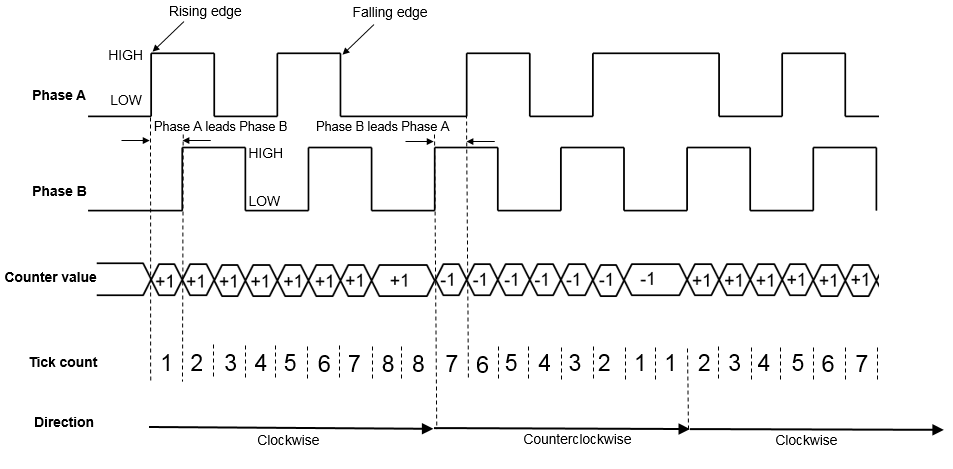
\includegraphics[width=\textwidth]{images/x4_encoder.png}
    \caption{Encoder in quadratura con risoluzione X4}
    \label{fig:x4_encoder}
\end{figure}

La risoluzione degli encoder è di 500 pulsazioni al giro, e sappiamo che al motore è collegata una riduzione 1:74, quindi possiamo ricavare quanti tick corrispondano ad un giro della ruota:

\begin{displaymath}
TicksPerGiro = Pulsazioni Encoder * Risoluzione Encoder * Riduzione = 148000
\end{displaymath}

Misurando la circonferenza delle ruote abbiamo tutti i dati necessari per calcolare la velocità per ogni ruota in m/s.

\subsubsection{Calcolo velocità}

È stata creata una classe per leggere gli encoder e calcolare la velocità delle ruote, nella quale sono memorizzati il puntatore alla periferica timer, il numero di tick per giro di ruota, la circonferenza delle ruote, i tick letti, i millisecondi passati dall'ultima lettura e i millisecondi passati al momento della lettura corrente.

\begin{figure}[htb]
    \centering
    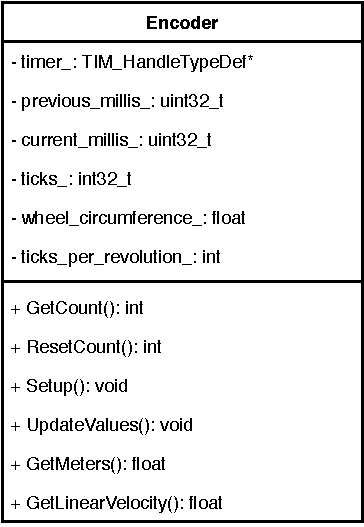
\includegraphics[scale=0.80]{images/encoder_class.pdf}
    \caption{Diagramma UML della classe Encoder}
    \label{fig:encoder_class}
\end{figure}

Innanzitutto occorre effettuare la configurazione del timer all'inizio del programma, avviando la periferica e impostando il valore registro CNT a metà del valore massimo in modo che, quando si va a leggere il valore del registro, si possa distinguere se l'encoder stia girando in senso orario o antiorario. Si memorizzano inoltre i millisecondi passati dall'inizio del programma.

Attraverso la funzione GetCount() andiamo a leggere il valore del registro CNT, e lo sottraiamo dalla metà del valore massimo che può assumere il registro: in questo modo se il valore ritornato è positivo sappiamo che la ruota sta girando in senso orario, se il valore è negativo sappiamo che la ruota sta girando in senso antiorario. Ad ogni lettura andiamo a resettare il valore di CNT alla metà del suo valore massimo attraverso la funzione ResetCount().
Chiamando la funzione UpdateValues() andiamo leggere e resettare il valore di CNT, e aggiorniamo i valori dei millisecondi passati dall'ultima chiamata alla funzione e i millisecondi correnti.
Per calcolare la distanza percorsa attraverso la funzione GetMeters() moltiplichiamo il numero di tick letti per circonferenza della ruota e dividiamo il tutto per il numero di tick per giro di ruota: in questo modo otteniamo i metri percorsi.
La funzione GetLinearVelocity() chiama le funzioni precedentemente definite, calcola la differenza tra il numero di millisecondi trascorsi tra la lettura in corso e la lettura precedente e quindi calcola la velocità in metri al secondo dividendo i metri percorsi per il numero di secondi passati dall'ultima lettura e otteniamo la velocità attuale della ruota in m/s. Questa funzione viene poi usata sia per il calcolo dell'odometria, sia per calcolare l'errore rispetto al setpoint nel loop PID.

\subsection{Controllo PID dei motori}

\subsubsection{Gestione motor driver}

Per poter controllare i motori tramite un microcontrollore bisogna utilizzare elettronica aggiuntiva, ovvero il motor driver, in quanto il segnale generato dal microcontrollore non è sufficiente per guidare un motore: il microcontrollore non è in grado di erogare tensione e corrente sufficienti.
Il motor driver è in grado, dati gli adeguati input, di erogare in output tensione e corrente adeguate per guidare il motore.

Il motor driver opera erogando una tensione al motore, la velocità è proporzionale al valore della tensione. Attraverso il segnale digitale PWM si può modulare la tensione, per simulare un segnale analogico, la cui tensione sarà pari a $V_{max}*Duty Cycle$. 
Si può inoltre controllare la direzione del movimento in base alla polarità della tensione applicata. Nel caso in cui non venga applicata alcuna tensione al motore esso è libero di ruotare.

Per controllare il motor driver è stata usata la modalità \textit{sign-magnitude}, ovvero un segnale PWM è utilizzato per regolare la velocità del motore, mentre un pin di direzione inverte la polarità della tensione (e quindi la direzione nella quale il motore sta girando) a seconda che il segnale sia alto o basso. Per il controllo di ciascun motore sono necessari 3 pin: un pin per la direzione, un pin per il PWM e un pin di sleep, usato nel caso in cui si voglia lasciare libero il motore.

Il segnale PWM (figura \ref{fig:pwm}) è un particolare tipo di segnale caratterizzato da una frequenza e un duty cyle. Per la generazione dei due segnali PWM sono stati utilizzati due canali del timer TIM4.
La frequenza del timer è stata impostata a 20 kHz come da datasheet, attraverso la seguente configurazione: 

\begin{displaymath}
TIM4 \; frequency = \frac{16 MHz}{(0 + 1)*(799 + 1)} = 20 kHz
\end{displaymath}

I canali 3 e 4 del TIM4 sono stati impostati in modalità PWM 1: in questa modalità il registro CNT viene incrmentato a ogni tick del timer e il segnale in uscita del canale x viene mantenuto alto fintanto che il registro CNT < registro CCRx. Per controllare il duty cycle del PWM viene quindi impostato il valore del registro CCRx, che varia tra 0 (duty cycle allo 0\%) e il valore contenuto nel registro ARR (duty cycle al 100\%).

È stata quindi creata la classe MotorController, nella quale sono contenuti i riferimenti ai pin da usare e i metodi per controllare il motore.
Sono stati scritti i seguenti metodi:
\begin{itemize}
    \item SetSpeed(int): imposta il duty cycle del PWM al valore passato in ingresso. Se il valore passato in ingresso è positivo il pin DIR è settato ad alto (motore gira in avanti), se il valore è negativo il pin DIR è settato a basso (motore gira indietro).
    \item Brake(): imposta il duty cycle del pwm a 0. In questo modo il motore viene frenato.
    \item Coast(): imposta il pin sleep a basso, scollegando così l'alimentazione al motore, in modo da farlo girare liberamente.
\end{itemize}

\begin{figure}[ht]
    \centering
    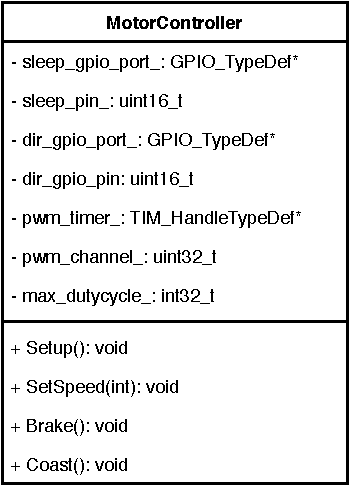
\includegraphics[scale=0.80]{images/motorcontroller_class.pdf}
    \caption{Diagramma UML della classe MotorController}
    \label{fig:motorcontroller_class}
\end{figure}

\subsubsection{Controllo PID}

Il controllo effettivo dei motori è gestito tramite loop di controllo PID. 
Il controllo PID è un sistema con retroazione negativa, ovvero l'output del controllore, che viene dato in input al sistema da controllare, è ottenuto tramite la differenza tra il setpoint (lo stato da raggiungere) e lo stato corrente, stimato attraverso appositi sensori. Questa differenza è chiamata \textit{errore}.
La sigla PID sta per Proporzionale-Integrale-Derivativo: questo tipo di controllore opera sull'errore attraverso le seguenti parti:
\begin{itemize}
    \item Parte \textbf{proporzionale} dove l'errore corrente viene moltiplicato per un gain \textit{kp}
    \item Parte \textbf{integrale} dove i vari errori vengono accumulati nel tempo, questo valore viene poi moltiplicato per un gain \textit{ki}
    \item Parte \textbf{derivativa} dove la derivata dell'errore viene moltiplicata per un gain \textit{kd}
\end{itemize}

Le tre parti ottenute vengono poi sommate, e si ottiene l'output da dare come comando al sistema da controllare. Questo è valido per un sistema a tempo continuo, ma usando un microcontrollore ci troviamo in un sistema a tempo discreto, quindi l'integrale diventa la sommatoria di tutti i valori campionati dell'errore e la derivata diventa la differenza tra l'errore corrente e l'ultimo errore campionato.

Il controllo PID deve avvenire ad una frequenza costante, per questo motivo è stato sfruttato il timer TIM6 per generare un interrupt periodico a 100 Hz, nella cui callback opera il sistema di controllo.

È stato adottato un sistema di controllo cross-coupling \cite{cross_pid}: in questo sistema abbiamo due loop di controllo indipendenti per il motore destro e il motore sinistro, e un loop di controllo aggiuntivo che opera sulla differenza tra le velocità dei due motori. I controllori sui singoli motori sono, come tutti i controllori, soggetti a errori e non permettono di raggiungere perfettamente i setpoint: la direzione di movimento del robot varia in base alla differenza di velocità tra i due motori, per questo motivo senza un controllo incrociato il robot potrebbe curvare più o meno di quanto si desidera. Con il controllo cross-coupling è possibile minimizzare l'errore più significativo, ovvero l'errore di orientamento del robot.
Il setpoint del sistema cross-coupling è la differenza voluta tra la velocità delle ruote, ad esempio se si vuole che il robot proceda dritto la differenza voluta tra le velocità sarà 0. Come in ogni controllore PID viene calcolato l'errore tra il setpoint e la misura corrente dello stato, e viene calcolato l'output come precedentemente spiegato. L'output del controllore cross-coupling viene poi sommato all'output del controllore del motore destro e sottratto dall'output del controllore del motore sinistro. I due output destro e sinistro così ottenuti vengono poi mandati in input al ponte H.

Dopo la progettazione del sistema segue la fase di calibrazione dei PID, in cui bisogna trovare le costanti di guadagno \textit{kp, ki, kd} di ogni sistema di controllo. Non avendo a disposizione il modello matematico dei sistemi da controllare non è stato possibile un approccio analitico, si è quindi usato un metodo empirico.

È stato scritto un apposito script python per il tuning: all'avvio dello script vengono chiesti in input qual è il controllore che si vuole calibrare (destro, sinistro o cross-coupling), il setpoint desiderato e le tre costanti kp, ki, kd. Questi parametri vengono inviati al microcontrollore che imposta i parametri del PID scelto. Alla pressione di un bottone presente sulla scheda viene avviato il controllore PID e vengono periodicamente inviati i dati degli encoder al computer. In questo modo è possibile monitorare l'andamento dello stato del sistema e farne un plot. Le costanti di guadagno vengono impostate in modo tale da poter raggiungere velocemente il setpoint, ma allo stesso tempo non superarlo troppo, e ritornare velocemente al setpoint anche in presenza di disturbi. 

\begin{figure}[H]
    \centering
    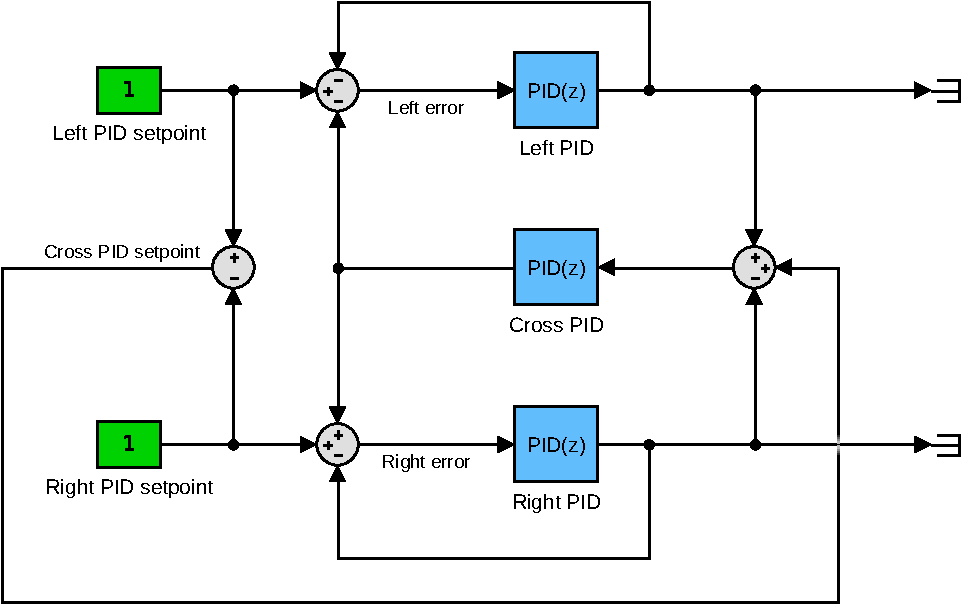
\includegraphics[width=\textwidth]{images/crosspid.pdf}
    \caption{Schema a blocchi del sistema}
    \label{fig:pid}
\end{figure}

\subsection{Comunicazione seriale con computer}

\subsubsection{Periferica UART}
La comunicazione con il computer di controllo è effettuata tramite la periferica UART (Universal Asynchronous Receiver-Transmitter). In particolare viene usata la periferica USART6 con la seguente configurazione:

\begin{itemize}
    \item Baud Rate: 9600 bit/s
    \item Word Length: 8 bit
    \item Parity: None
    \item Stop Bits: 1 bit
    \item Hardware Flow Control: RTS only
\end{itemize}

Descriviamo il protocollo UART. Se non si stanno inviando dati il livello del segnale è tenuto alto, quando si trasmette un data frame si inizia la comunicazione con uno start bit, ovvero un bit uguale a zero (livello del segnale basso). Successivamente si inviano i bit contenenti l'informazione da trasmettere, nel nostro caso 8 bit. La trasmissione del data frame si conclude con uno stop bit, ovvero un bit uguale a 1. Essendo UART un protocollo asincrono, ovvero senza un clock, il ricevente usa start bit e stop bit per poter effettuare il sampling del segnale, sapendo che $durata\_bit = 1/baud rate$

L'Hardware Flow Control permette di controllare il flusso di dati via hardware. Nello specifico abbiamo la modalità RTS (Request To Send) only: ciò significa che sulla scheda Nucleo ci sarà un pin di output a cui viene attribuita la funzione di RTS, e questo pin verrà poi collegato all'input CTS (Clear To Send) del modulo seriale. Il pin RTS viene automaticamente settato al livello logico alto se la periferica UART della scheda Nucleo è pronta a ricevere dati, in caso contrario il pin è settato al livello logico basso. In questo modo il computer che sta inviando dati all'UART può inviare i dati solo quando la scheda Nucleo è pronta a riceverli.

La comunicazione nel nostro caso è full-duplex, ovvero abbiamo linee separate per la ricezione e la trasmissione di dati.

\begin{figure}[htb]
    \centering
    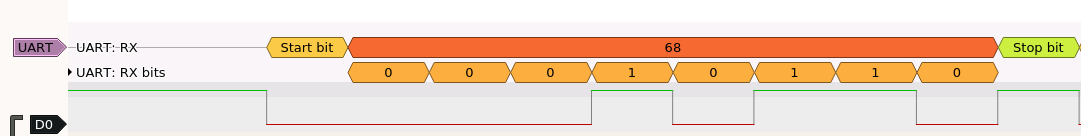
\includegraphics[width=\textwidth]{images/uart_protocol.png}
    \caption{Segnale UART, visualizzato tramite un analizzatore logico con il software Pulseview}
    \label{fig:uart_protocol}
\end{figure}

\subsubsection{Periferica DMA}
Come modalità di input/output si è scelto l'accesso diretto alla memoria grazie alla periferica DMA.
Il DMA permette di trasferire dati in background, senza l'intervento del processore. Durante questi trasferimenti la CPU è libera di proseguire l'esecuzione del programma, alla fine del trasferimento viene generato un interrupt dal DMA per segnalare alla CPU che l'operazione è terminata.
Il DMA controller presenta più stream, ed ogni stream ha collegati più canali. Ogni canale corrisponde ad una specifica periferica, che viene selezionata in fase di configurazione.
Nel nostro caso vengono usati due stream, uno per la ricezione dei dati dall'UART e uno per l'invio dei dati dall'UART.

Usiamo la periferica DMA2 in quanto è quella collegata ad USART6 e usiamo due stream, uno per la ricezione e uno per la trasmissione.

\begin{listing}[H]
\inputminted[frame=single,framesep=10pt]{c}{codice/dma2_rx_config.c}
\caption{Configurazione dello stream di ricezione}
\label{listing:DMA_rx_config}
\end{listing}

In questo modo stiamo settando lo stream 1, dicendo di usare il canale 5 ovvero il canale collegato a USART6\_RX. La direzione PERIPH\_TO\_MEMORY indica che il DMA trasferirà i dati dalla periferica alla memoria: abbiamo che il DMA trasferirà i dati dal registro della periferica USART contenente il byte ricevuto ad un buffer in memoria. Il parametro DMA\_MINC\_ENABLE fa si che l'indirizzo del buffer in memoria viene incrementato automaticamente dal DMA. 
La modalità è circolare, in modo da poter gestire la ricezione continua dei dati: se si arriva alla fine del buffer in memoria si ricomincia dall'inizio.

\begin{listing}[H]
\inputminted[frame=single,framesep=10pt]{c}{codice/dma2_tx_config.c}
\caption{Configurazione dello stream di trasmissione}
\label{listing:DMA_tx_config}
\end{listing}

In questo modo stiamo settando lo stream 6, dicendo di usare il canale 5 ovvero il canale collegato a USART6\_TX. La direzione MEMORY\_TO\_PERIPH indica che il DMA trasferirà i dati dalla memoria alla periferica: abbiamo che il DMA trasferirà i dati dal buffer di trasmissione in memoria al registro della periferica USART contenente il byte da inviare. Il parametro DMA\_MINC\_ENABLE fa si che l'indirizzo del buffer in memoria viene incrementato automaticamente dal DMA. 

In entrambe le configurazioni la priorità è impostata a LOW: avere la stessa priorità significa che nel caso avvengano due richieste del DMA contemporaneamente verrà prima gestita quella dello stream con numero minore, in questo caso lo stream 1.

\subsubsection{Serializzazione dati}
Per la trasmissione e la ricezione dei dati si è scelto di usare il protocollo di serializzazione Protocol Buffers. In questo modo viene garantita l'indipendenza da piattaforme e linguaggi specifici per quanto riguarda il lato computer: non si è infatti legati ad una specifica rappresentazione dei bit 
in quanto i dati vengono serializzati e la libreria è disponibile per diversi linguaggi di programmazione. Nello specifico sul microcontrollore è stato utilizzato \textit{nanopb}, un'implementazione specifica per i microcontrollori a 32 bit e per i sistemi con memoria limitata.

Innanzitutto è necessario specificare la struttura dei messaggi in un file di tipo .proto, utilizzando la sintassi specifica di Protocol Buffer che è indipendente da linguaggi specifici. Sono stati definiti due messaggi: StatusMessage, per l'invio di dati dal robot al computer, e VelocityCommand, per l'invio dei comandi di velocità dal computer al robot.

StatusMessage contiene velocità lineare e velocità angolari correnti, i millisecondi passati dal precedente invio del messaggio e un codice di status.

VelocityCommand contiene la velocità lineare e la velocità angolare da raggiungere.

\begin{listing}[H]
\lstinputlisting[language=protobuf2, 
                style=protobuf,
                captionpos=b]{codice/otto_communication.proto}
\caption{Definizione dei messaggi con Protocol Buffers}
\label{listing:protobuf_definition}
\end{listing}


Dopo aver definito la struttura dei messaggi nel file .proto bisogna generare i file da includere nel codice del microcontrollore: tramite uno script python vengono generati i file .pb.h e .pb.c, contenenti le struct che rappresentano i messaggi. Oltre ai file generati dal .proto è necessario includere i file generali per codifica e decodifica che contengono i metodi per effettuare serializzazione e deserializzazione degli stream di dati.

\subsubsection{Invio dati}
L'invio dei dati è effettuato ad una frequenza costante come precedentemente spiegato: il timer TIM6 genera un interrupt a frequenza 10Hz, nella callback di questo interrupt gestiamo l'invio dei dati.

Nella callback vengono lette le velocità delle ruote, e vengono calcolate velocità lineare e velocità angolare con la funzione FromWheelToOdom(float left\_wheel\_velocity, float right\_wheel\_velocity) della classe Odometry, che prende in input le due velocità delle ruote. Vengono letti i millisecondi trascorsi dall'avvio, da cui sottraiamo i millisecondi trascorsi dall'avvio letti all'invio del messaggio precedente, così da avere i millisecondi trascorsi dall'ultimo invio. Impostiamo inoltre il campo \textit{status} uguale a 3, corrispondente allo stato \textit{running}.
Possiamo quindi procedere alla serializzazione del messaggio attraverso la funzione pb\_encode e avviare la trasmissione UART in modalità DMA dello stream ottenuto dalla serializzazione tramite la funzione delle librerie di hardware abstraction layer HAL\_UART\_Transmit\_DMA.

Inviamo il messaggio StatusMessage anche nel caso vengano rilevati dei fault dei motori, nella callback dell'interrupt ad essi legata: in questo caso il codice di status sarà 4 o 5 a seconda del fault rilevato.


\begin{listing}[H]
\inputminted[frame=single,framesep=10pt]{cpp}{codice/dma_tx_code.cpp}
\caption{Codice per la trasmissione dell'odometria}
\label{listing:trasmissione_dati}
\end{listing}


\subsubsection{Ricezione comandi}
La ricezione dei comandi è sempre gestita in modalità DMA: all'inizio del programma, dopo aver configurato tutte le periferiche si configura la periferica UART per ricevere un numero di byte corrispondente alla lunghezza del messaggio VelocityCommand attraveso la funzione HAL\_UART\_Receive\_DMA. In questo modo quando viene ricevuto quel numero di byte la periferica genera un interrupt a cui corrisponde la callback HAL\_UART\_RxCpltCallback.
In questa callback ci occupiamo di decodificare i byte ricevuti: nel caso la decodifica abbia successo significa che i byte sono stati inviati e ricevuti correttamente e possiamo quindi procedere all'elaborazione del comando ricevuto, nel caso la decodifica fallisca scartiamo il messaggio.
Quando riceviamo correttamente un messaggio procediamo a ricavare da velocità lineare e angolare i setpoint per la velocità delle ruote con la funzione FromCmdVelToSetpoint(). Impostiamo quindi i setpoint dei PID delle singole ruote e il setpoint del PID che gestisce la differenza tra la velocità delle ruote.
Reimpostiamo infine la periferica per generare l'interrupt con la funzione HAL\_UART\_Receive\_DMA.


\begin{listing}[H]
\inputminted[frame=single,framesep=10pt]{cpp}{codice/dma_rx_code.cpp}
\caption{Codice relativo alla ricezione dei comandi}
\label{listing:ricezione_dati}
\end{listing}


\section{Implementazione nodo ROS sul computer}
Per quanto riguarda la gestione da parte del computer di controllo è stato scritto il nodo ROS \textit{serial\_bridge} in python che si occupa di:

\begin{itemize}
    \item Ricevere i messaggi dal robot.
    \item Calcolare l'odometria e pubblicare i messaggi ad essa relativi.
    \item Trasmettere i comandi di velocità al robot.
\end{itemize}

\subsubsection{Codice python}
Innanzitutto il nodo resta in attesa di poter aprire la porta seriale. Quando la porta seriale è disponibile viene aperta, e viene effettuato il reset della scheda Nucleo tramite il pin DTR del modulo seriale, che è collegato al pin NRST della scheda Nucleo.

Dopo l'apertura della porta seriale il nodo si sottoscrive al topic \textit{/cmd\_vel} e crea il publisher per i topic \textit{/odom} e \textit{tf}.

Il nodo resta quindi in attesa di ricevere dati dalla porta seriale, in particolare aspetta di ricevere un numero di byte pari alla lunghezza del messaggio \textit{otto\_status}. Quando questi byte vengono ricevuti si procede con la decodifica del messaggio: nel caso in cui lo status del messaggio sia 3 (ovvero \textit{running}) si procede con il calcolo dell'odometria e la pubblicazione dei messaggi ROS ad essa relativi, nel caso lo status sia 4 o 5 (quindi è stato rilevato un malfunzionamento) viene pubblicato un messaggio di errore.

Ogni volta che viene ricevuto un messaggio sul topic \textit{/cmd\_vel} viene effettuata una callback, nella quale il messaggio ricevuto viene serializzato attraverso la libreria Protocol Buffers. Viene poi controllato lo stato del pin CTS, ovvero si controlla se la scheda Nucleo sia pronta a ricevere un messaggio: in caso positivo viene inviato il messaggio serializzato, altrimenti viene pubblicato un messaggio di warning.

Quando il nodo riceve un segnale di shutdown prima di terminare procede al reset della scheda Nucleo tramite il pin DTR per questioni di sicurezza.

\subsubsection{Calcolo odometria}
A partire dalla velocità lineare e la velocità angolare trasmesse dal robot è possibile ricavare una stima della sua pose a partire dalla sua pose precedente: questo metodo è chiamato \textit{dead reckoning}.
Usiamo un sistema in cui ci sono 3 gradi di libertà, ovvero stimiamo le pose sul piano. La pose sarà quindi descritta come $[x,y,\theta]^T$
Si prende come sistema di riferimento la prima pose del robot, quindi si parte dalla pose $[0,0,0]^T$.

Le seguenti formule, relative al calcolo della pose di un robot a guida differenziale, vengono applicate ogni volta che si riceve un messaggio per calcolare la nuova pose.

Indichiamo con $\omega$ la velocità angolare, con $V$ la velocità lineare, con $\delta t$ i secondi passati, con $[x,y,\theta]^T$ la pose attuale e con $[x',y',\theta']^T$ la nuova pose calcolata.

Per semplicità del codice distinguiamo due casi: il caso in cui il robot stia percorrendo una curva con raggio infinito e il caso in cui stia percorrendo una curva con raggio finito.

Nel primo caso il robot sta percorrendo una linea dritta, quindi possiamo semplicemente sommare i metri percorsi alla pose precedente, tenendo conto dell'orientamento rispetto al mondo.

%caso dritto
\begin{displaymath}
    \begin{bmatrix} x' \\ y' \\ \theta'  \end{bmatrix}
    =
    \begin{bmatrix} 
        x+\cos(\theta)\cdot(V\cdot\delta t) \\ 
        y+\sin(\theta)\cdot(V\cdot\delta t) \\ 
        \theta  
    \end{bmatrix}
\end{displaymath}

Nel secondo caso il robot sta percorrendo un arco della circonferenza che ha centro in ICC (centro di rotazione istantanea) e raggio R. A partire da velocità lineare e angolare possiamo ricavare il raggio e la posizione dell'ICC. Avendo a disposizione l'ICC calcoliamo la nuova pose traslando il robot in ICC, ruotiamo di $\delta \theta$ e infine ri-trasliamo al punto di partenza.

%ICC
\begin{displaymath}
    \begin{bmatrix}
        ICC_x \\
        ICC_y \\
    \end{bmatrix}
    =
    \begin{bmatrix}
        x - R \cdot \sin(\theta) \\
        y + R \cdot \cos(\theta) \\
    \end{bmatrix} \\
    \quad con \quad
    R = \frac{V}{\omega}
\end{displaymath}

%matrici finali
\begin{displaymath}
    \begin{bmatrix} x' \\ y' \\ \theta'  \end{bmatrix}
    =
    \begin{bmatrix}
        \cos(\omega \cdot \delta t) & -\sin(\omega \cdot \delta t) & 0 \\
        \sin(\omega \cdot \delta t) & \cos(\omega \cdot \delta t) & 0 \\
        0 & 0 & 1
    \end{bmatrix}
    \begin{bmatrix}
        x - ICC_x \\
        y - ICC_y \\
        \theta
    \end{bmatrix}
    +
    \begin{bmatrix}
        ICC_x \\
        ICC_y \\
        \omega \cdot \delta t
   \end{bmatrix}
\end{displaymath}

\section{Testing}
Il robot è stato testato in ambiente reale per verificarne il corretto funzionamento.

Innanzitutto è stato scritto un nodo ROS in python, \textit{joypad\_bridge}, che permette di trasmettere messaggi sul topic \textit{/cmd\_vel} tramite un joypad USB collegato al computer: con l'analogico sinistro si controlla la velocità lineare del robot, con l'analogico destro la velocità angolare.
In questo modo è stata verificata la corretta ricezione dei comandi di velocità da parte del robot e la loro corretta esecuzione.

Sfruttando il nodo \textit{joypad\_bridge} è stato poi possibile effettuare dei test per quanto riguarda l'odometria del robot. Dopo aver confermato la corretta ricezione dei messaggi contenenti i dati di odometria sul computer è stato usato il tool RVIZ per verificare l'accuratezza dei calcoli relativi all'odometria. Il robot è stato guidato attraverso un percorso ad anello (quindi con partenza e arrivo nello stesso punto) di circa 10 metri, che comprendeva curve, rettilinei e giri su sé stesso: sono stati visualizzate le pose ottenute tramite RVIZ, e si è confrontata la pose iniziale con quella finale. È stato misurato un errore di circa 40 centimetri, considerato accettabile in quanto gli encoder non tengono conto degli slittamenti delle ruote (in quanto misurano soltanto i giri del motore) e il calcolo dead reckoning è soggetto all'accumulo degli errori precedenti.
\chapter{Conclusioni}

L’obiettivo di questo lavoro è stato lo studio e lo sviluppo di un sistema di controllo per una base robotica, che possa poi essere utilizzata per la ricerca in ambito di guida autonoma e percezione outdoor.

La base robotica era già presente in laboratorio IRA, tuttavia mancava dei componenti elettronici per poter essere utlizizzabile.
Innanzitutto è stato quindi necessario fare un'analisi dei requisiti hardware, acqusistare i componenti mancanti e procedere alla loro installazione fisica sulla base robotica.

È stato poi sviluppato il software di basso livello per interagire con i sensori e gli attuatori presenti sulla base robotica, in modo da poter controllare i motori e leggere le velocità delle ruote.

Ha avuto grande rilievo lo studio della comunicazione tra il microcontrollore e il computer di controllo, in modo da poter comandare il robot dal computer tramite il framework ROS. Sono stati sviluppati sia la parte di comunicazione a basso livello tra microcontrollore e computer, sia un nodo ROS in python in grado di ricavare l'odometria a partire dai dati degli encoder e di trasmettere comandi di velocità al robot.

Il tutto è stato poi testato usando un joypad collegato al compuer per l'invio dei comandi al robot e visualizzando l'odometria ricavata tramite lo strumento RVIZ. 

Il sistema di controllo si è dimostrato funzionante, e Otto potrà quindi essere utilizzato in futuro, aggiungendo sensori eterocettivi, per esperimenti e ricerca all'interno del laboratorio.




\newpage
\printbibheading[heading=bibintoc, title={Riferimenti}]
\printbibliography[nottype=online,heading=subbibintoc,title={Bibliografia}]
\printbibliography[type=online,heading=subbibintoc,title={Siti}]

\appendix
\chapter{Lista delle parti}

\textbf{Base robotica:}
\begin{itemize}
    \item Base robotica Volksbot RT 3
    \item Dimensioni: 580 x 520 x 315 mm
    \item Dimensione baseline: 435 mm
    \item Peso (escluse batterie): 17kg
    \item Ruote 260 x 85 mm, ruota di supporto piroettante 200mm
    \item Circonferenza ruote misurato a 3 bar: 783mm
    \item Batterie al piombo 12V, 15AH
\end{itemize}
\textbf{Motori:}
\begin{itemize}
    \item Motori Maxon RE 40 Ø40 mm, Graphite Brushes, 150 Watt
    \item Riduzioni 1:74 Planetary Gearhead GP 42 C Ø42 mm, 3 - 15 Nm, Ceramic Version
    \item Encoder HEDS-5540\#A11
\end{itemize}
\textbf{Elettronica:}
\begin{itemize}
    \item Scheda di controllo Nucleo F767ZI
    \item Modulo seriale FTDI FT232RL
    \item Motor driver Pololu Dual G2 High-Power Motor Driver 24v18 Shield
    \item PCB custom disegnata con KiCad, disponibile sulla repo del progetto
\end{itemize}

\end{document}
